\section{Experimento}

\begin{frame}
  \frametitle{Amostragem}
  Características dos locais amostrados (2007 e 2008):
  \begin{itemize}
	  \item Residencial (\ang{+5;35;2.00} e \ang{-0;11.;58}):
	  Avenida com pouco tráfego de veículos e não pavimentada
  \item Tráfego (\ang{+5;34;54} e \ang{-0;11;56.30}):
	  Avenida pavimentada com tráfego intenso de veículos (com exceção do período noturno).
  \end{itemize}
\end{frame}

\begin{frame}
  \frametitle{Pontos de amostragem em Nima}
  \begin{figure}[H]
    \centering
    \caption{Amostragem Nima}
    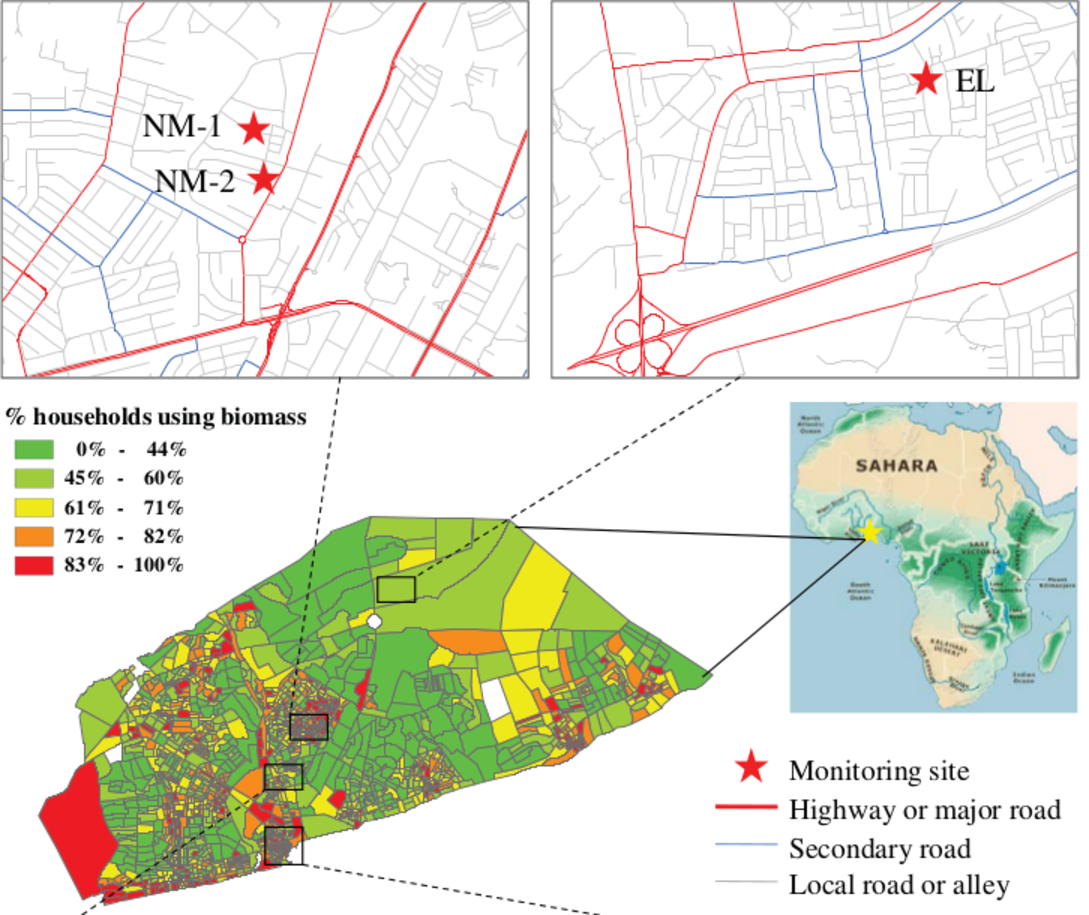
\includegraphics[scale=0.35]{../../../inputs/images/zheng/nima_mapa.pdf}
  \end{figure}
\end{frame}

\begin{frame}
  \frametitle{}
  \begin{figure}[H]
    \centering
      \includegraphics[scale=0.17]{../../../outputs/winter2006_2007.pdf}
      \includegraphics[scale=0.17]{../../../outputs/spring2007.pdf}
      \includegraphics[scale=0.17]{../../../outputs/summer2007.pdf}
  \end{figure}

  \begin{figure}[H]
    \centering
      \includegraphics[scale=0.17]{../../../outputs/autumn2007.pdf}
      \includegraphics[scale=0.17]{../../../outputs/harmattan2007_2008.pdf}
      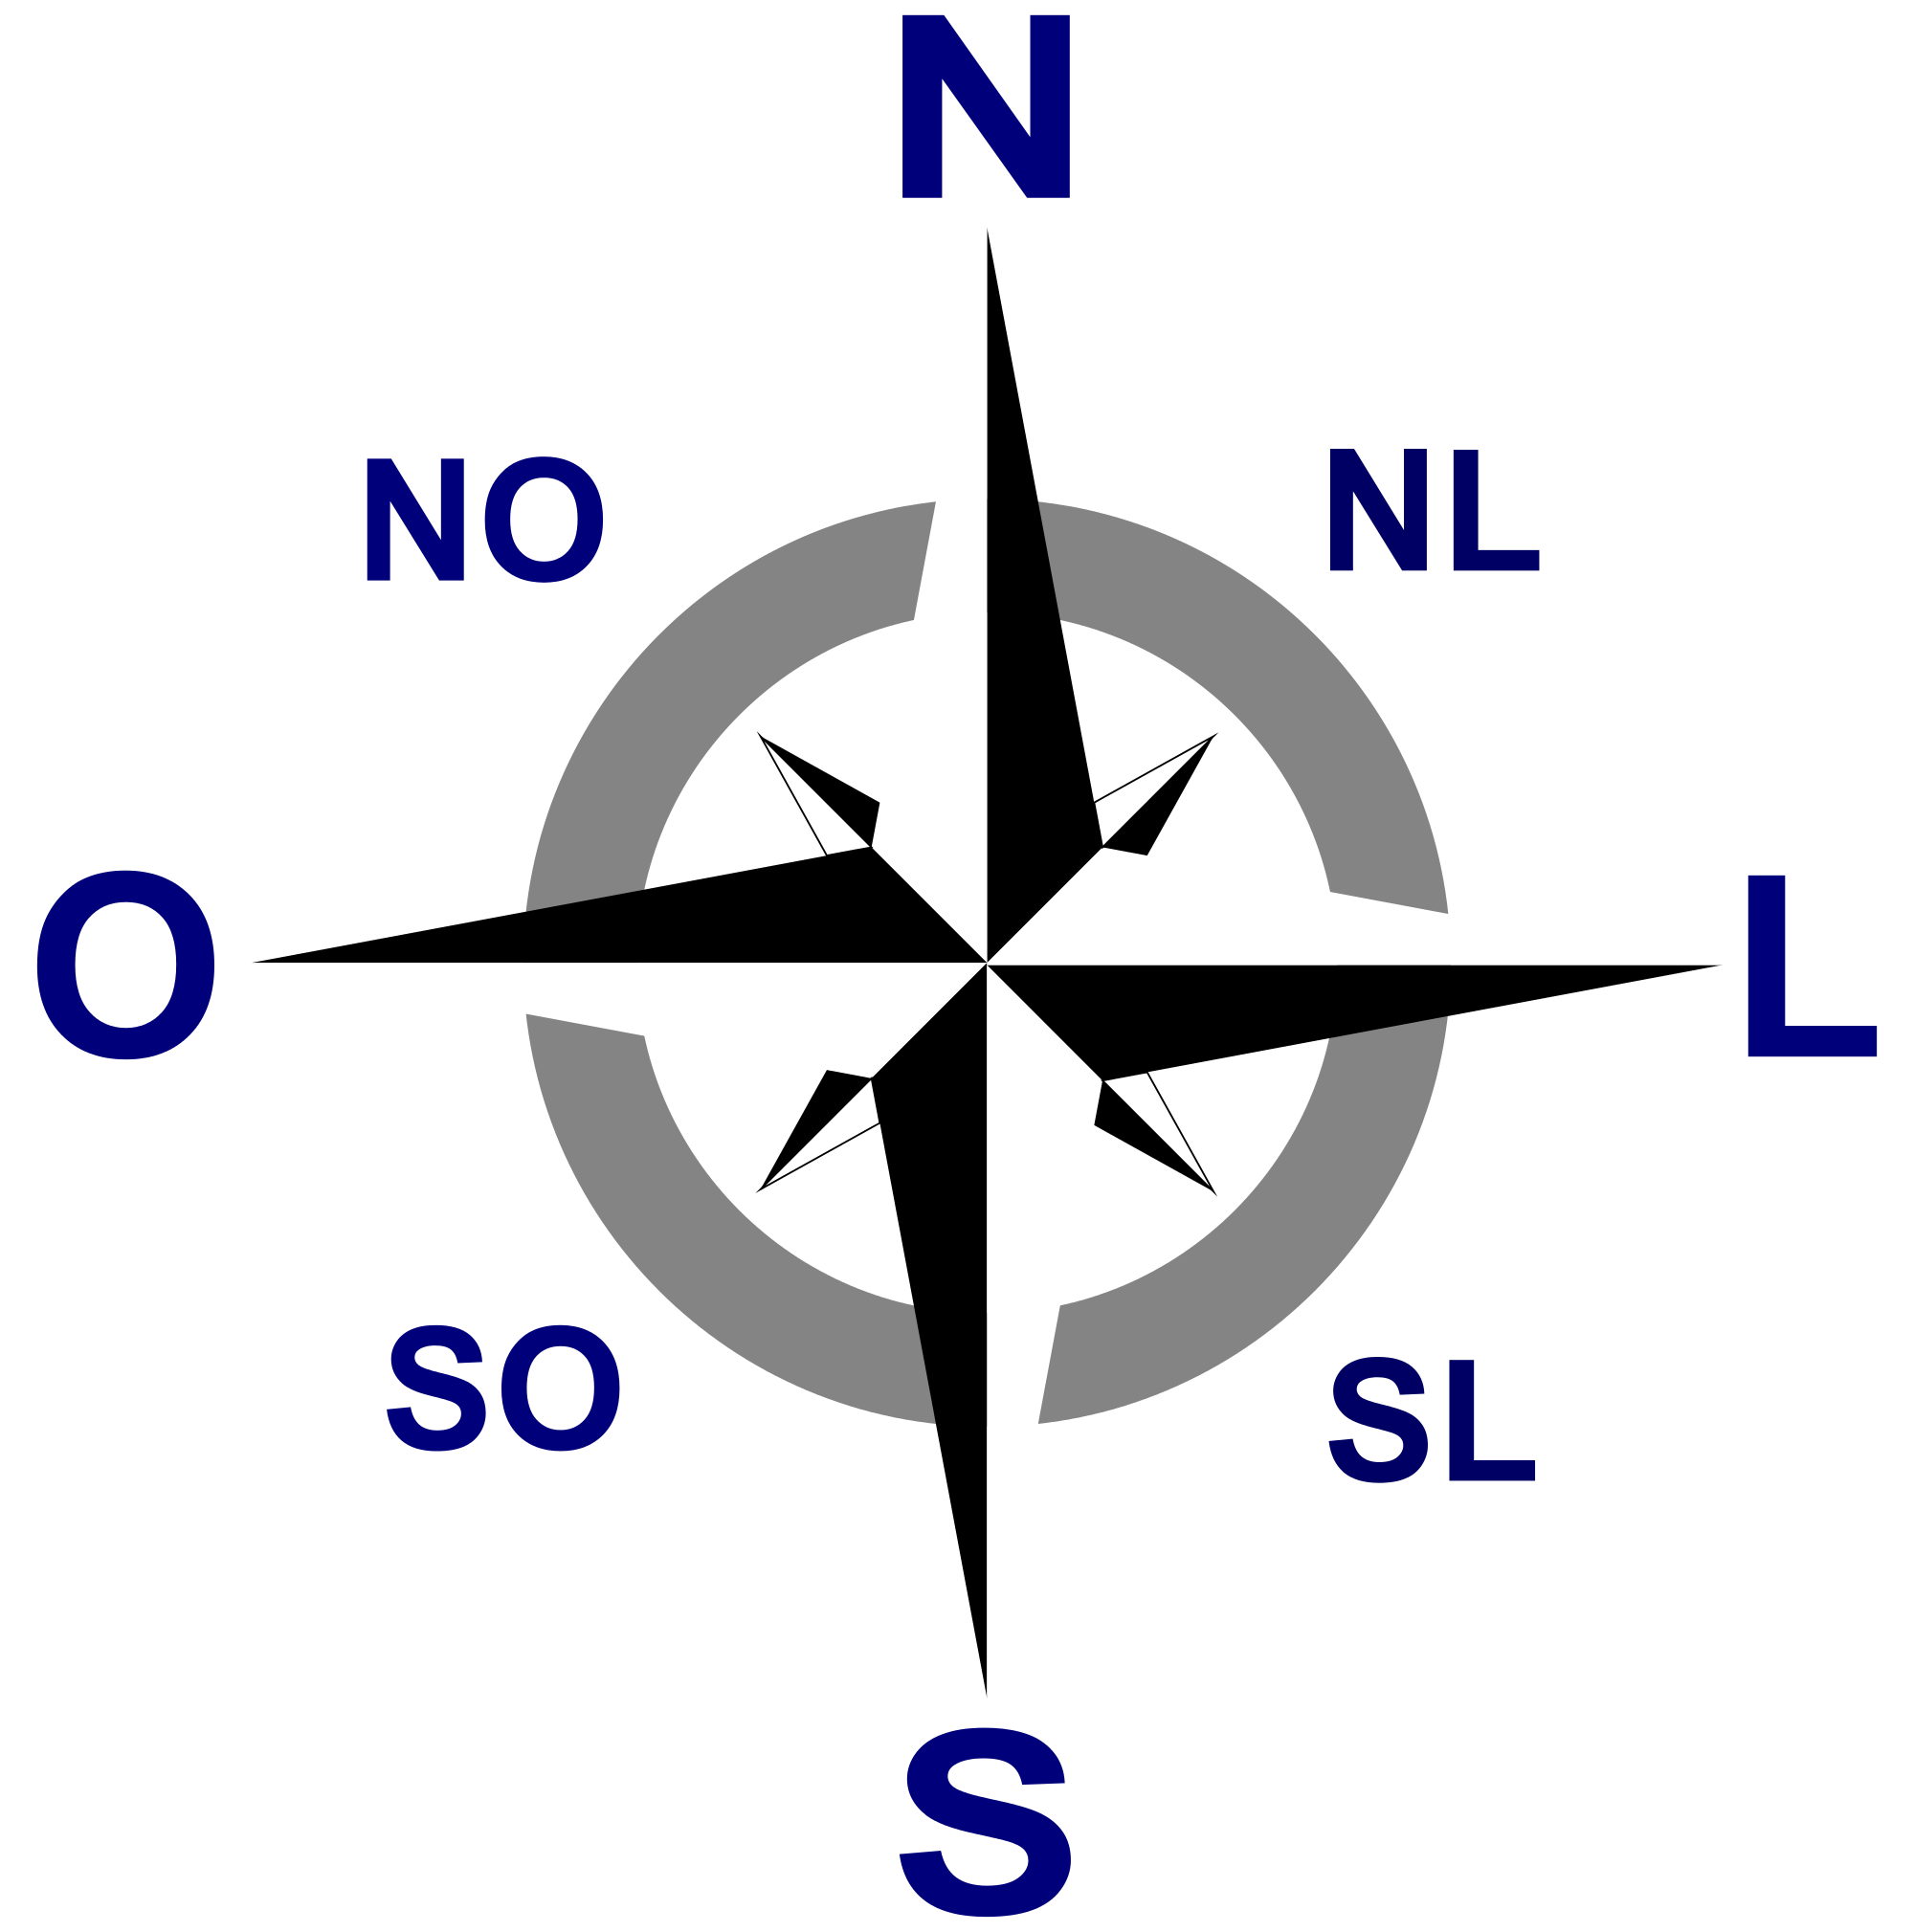
\includegraphics[width=1cm]{../../../inputs/images/rosa_ventos}
      \caption{Distribuição das frequência de direção dos ventos, dados da NOAA}
  \end{figure}
\end{frame}

\begin{frame}
  \frametitle{Fluorescência de Raios X - \textit{ED-XRF}}
  Modelamento matemático usado na \textit{ED-XRF}:
  \begin{equation}
	  N_{ij} \propto \frac{m_{ij}}{A_i}I_i{\Delta}t_{i}
  \end{equation}
  Onde,  
  \begin{itemize}
    \item $N_{ij}$ = Contagem de fótons na amostra i para o elemento químico j;
    \item $I_{i}$ = Corrente (ampère) na amostra i;
    \item $\Delta t_i$ = Tempo vivo (segundos) que a amostra i foi irradiada;
    \item \textcolor{red}{$m_{ij}$} = Massa (grama) na amostra i para o elemento químico j;
    \item $A_i$ = Área ($cm^2$)irradiada da amostra i.
  \end{itemize}
\end{frame}

\begin{frame}
  \frametitle{Calibração: Ajuste do Fator de Resposta}
  Constante de proporcionalidade: Fator de Resposta:
  \begin{equation}
    R_j = \frac{A_i}{m_{ij}} \frac{N_{ij}}{I_i \Delta t_i}
  \end{equation}
  \begin{figure}[H]
  \centering
    \begin{minipage}[b]{0.40\linewidth}
      \includegraphics[scale=0.25]{../../../outputs/K2014abril}
    \end{minipage}
    \quad
    \begin{minipage}[b]{0.40\linewidth}
      \includegraphics[scale=0.25]{../../../outputs/L2014abril.png}
    \end{minipage}
  \end{figure}
\end{frame}


\begin{frame}
  \frametitle{Limite de Detecção}
  \begin{figure}[H]
  \centering
    \begin{minipage}[b]{0.40\linewidth}
      \includegraphics[scale=0.3]{../../../outputs/limitDetectionK}
    \end{minipage}
    \quad
    \begin{minipage}[b]{0.40\linewidth}
      \includegraphics[scale=0.3]{../../../outputs/limitDetectionL}
    \end{minipage}
  \end{figure}
\end{frame}

